\subsection{Mc Caskill}

Summe über alle Strukturen 
\begin{equation}
	Z=\sum\limits_{S} e^{-\beta \cdot E_{S}}
\end{equation}

mit $\beta= {1 \over {R \cdot T}}$, $E_{s}$= Energie der Sturktur S (alle Strukturen),\\ R = Gaskonstante = $k \cdot N_{A}$, T = Temperatur
\\\\
\textbf{Dynamic Programming Ansatz:}\\
 - Energie von einer Base = 1 $\rightarrow e^0=1$

\begin{equation}
	Z(i,j)= \underbrace{Z(i+1,j)}_{ungepaart} + \underbrace{\sum\limits_{i < k \leq j} Z^{B}(i,k) \cdot Z(k+1,j)}_{gepaart}
\end{equation}

mit $Z^B=$Basenpaar zwischen i,k

\begin{equation}
Z^B(i,j)= \underbrace{\mathcal{H}(i,j)}_{Hairpin} + \underbrace{\sum\limits_{i < k < l < j} \mathcal{I}(i,j, k, l) \cdot Z^B(k,l)}_{Interior} +  \underbrace{\sum\limits_{i < k < j} Z^M(i+1,u-1) \cdot Z^{M1}(u,j-1) \cdot e^{-\beta \cdot {a(i,j)}}}_{Multiloop}
\end{equation}

mit a = Energie fürs Schließen des Multiloops
\\\\
\underline{Initialisierung:}\\
$Z^M=0; Z^{M1}=0; Z^B=0$
\\\\
$Z^M(i,j) =$ ungepaart + genau 1 Basenpaar + Erweiterung um 1 Basenpaar, also mindestens 2

\begin{equation}
	Z^M(i,j) = Z^M(i+1,j) \cdot e^{-\beta \cdot c} + \sum\limits_{i < k < j} Z^B(i,k) \cdot e^{-\beta \cdot b} \cdot e^{-\beta(j-k)c} + \sum\limits_{i < k < j} Z^B(i,k) \cdot e^{-\beta \cdot b} \cdot Z^M(k+1,j)
\end{equation}

mit b,c=Konstanten zum Schließen der gepaarten Basen
\\\\
$\rightarrow$ da $Z^M$ mit 0 initialisiert, kann zunächst $Z^B$ als einzelnes Basenpaar $"$aufgeschrieben$"$ werden, dann erst Erweiterung möglich
\\\\
$Z^{M1}(i,j)=Z^{M1}(i,j-1) \cdot e^{-\beta \cdot c} + Z^B(i,j) \cdot e^{-\beta \cdot b}$
\\\\
Ergebnis= 4 Matrizen: $Z, Z^B, Z^M, Z^{M1} \rightarrow$ Backtracking
\\\\
\textbf{Wahrscheinlichkeit für Basenpaare:}
\begin{equation}
p(i,j)={Z(i,j) \over Z}
\end{equation}
\\\\
mit Z(i,j) gegeben i,j
\\\\
\begin{equation}
Z(i,j)=\underbrace{Z^B(i,j)}_{innen} \cdot \underbrace{\widehat{Z}^B(i,j)}_{außen}
\end{equation}
mit $\widehat{Z}^B$: wie beim suboptimalen Falten (Zuker Suboptimals) $\rightarrow$ Verdoppelung der Sequenzen
\\\\
\begin{equation}
\widehat{Z}^B(i,j)= Z^B(j,n-i)
\end{equation}
\begin{center}
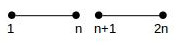
\includegraphics[width=0.4\textwidth]{lectures/160425/pix/1.jpg}
\end{center}
\textbf{teuer!}

\newpage

\begin{center}
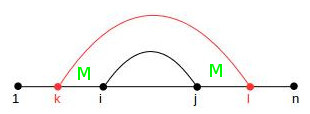
\includegraphics[width=0.7\textwidth]{lectures/160425/pix/2.jpg}
\end{center}
Achtung: Gleichung über mehrere Zeilen!
\\\\
\begin{tabular}{{cp{.5\linewidth}}}
  $\widehat{Z}^B(i,j)=Z(1,i-1) \cdot Z(j+1,n)\textbf{+}$ & i,j nicht von einem Basenpaar eingeschlossen\tabularnewline
  & \tabularnewline
  $\sum\limits_{k < i < j < l} \mathcal{I}(k,l,i,j) \cdot \widehat{Z}^B(k,l)\textbf{+}$ & i,j von einem Basenpaar k,l eingeschlossen (innerstes Basenpaar), kann kein Hairpin sein da Basenpaar i,j innen vorhanden\tabularnewline
  & \tabularnewline
  $\sum\limits_{k < i < j < l} \widehat{Z}^B(k,l) \cdot e^{-\beta \cdot b} \cdot e^{-\beta \cdot a} \cdot\textbf{\{}$ & \tabularnewline
  & \tabularnewline
  $Z^M(k+1,i-1) \cdot Z^M(j+1,l-1)\textbf{+}$ & Multiloop zwischen k und i \underline{und} j und l\tabularnewline
  & \tabularnewline
  $Z^M(k+1,i-1) \cdot e^{-\beta (l-j-1) \cdot c}\textbf{+}$& Multiloop nur zwischen k und i\tabularnewline
  & \tabularnewline
  $Z^M(j+1,l-1) \cdot e^{-\beta (j-k-1) \cdot c}\textbf{\}}$& Multiloop nur zwischen j und l\tabularnewline
\end{tabular}
\\\\
\\\\
Berechnung dauert $\mathcal O(n^4)$ da $k<i<j<l \rightarrow$ sehr teuer
\\\\
\textbf{$\Rightarrow$Verbesserung durch Multiloop-Berechnung}

\newpage

\underline{Definition:}\\\\
$Z^A(i,j)=\sum \limits_{j \leq k \leq n (=Ende)} \widehat{Z}^B(i,k) \cdot Z^M(j,k-1)$
\\\\
\begin{center}
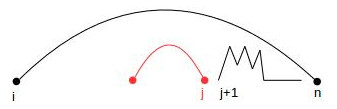
\includegraphics[width=0.6\textwidth]{lectures/160425/pix/3.jpg}
\end{center}
Ermittelt alle Zustandssummen, bei denen i mit n Multiloop schließt und innerhalb ein weiterer Multiloop existiert
\\\\
$Z^{A'}(i,j)=\sum \limits_{j \leq k \leq n} \widehat{Z}^B(i,k) \cdot e^{-\beta (k-j)}$
\\\\
wie oben aber ohne inneren Multiloop
\\\\
\textbf{$\Rightarrow$ damit:}
\\\\
\begin{tabular}{{cp{.5\linewidth}}}
  $\widehat{Z}^B(i,j)=...+ \sum \limits_{1 \leq k < i}Z^A(k,j+1) \cdot (Z^M(k+1,i-1))\textbf{+}$ & rechts und links Multiloop (gepaart)\tabularnewline
  & \tabularnewline
  $ \sum \limits_{1 \leq k < i}Z^A(k,j+1) \cdot e^{-\beta(k-i-1) \cdot c}\textbf{+}$ & nur rechts Multiloop (ungepaart)\tabularnewline
  & \tabularnewline
  $\sum \limits_{1 \leq k < i}Z^{A'}(k,j+1) \cdot (Z^M(k+1,i-1))$ & nur links Multiloop \tabularnewline
\end{tabular}
\\\\
\\\\
$\Rightarrow$ damit nur noch $\mathcal O(n^3)$\\
$\Rightarrow$ Anwendung der Berechneten Daten in Dotplot
\begin{itemize}
	\item Größe der Zellen repräsentiert Wahrscheinlichkeit für jedes Basenpaar
	\item Quadrat in Dotplot mit $\sqrt{p(i,j)}$ Seitenlänge
	\item in unterer Dreiecksmatrix mfe-Struktur (minimal free energy aus Zuker)
\end{itemize}

\textbf{Weitere Visualsierungsmöglichkeiten:}
\begin{itemize}
	\item Centroid: die Struktur, die von allen am wenigsten entfernt ist; alle Basenpaare, die mindestens $p \geq 0,5$ haben
	\item MEA-Struktur (maximum expected accuracy): z.B. Nussinov mit scores proportional zu p(i,j)
	\item Strukturplot mit Färbung proportional zur Basenpaar wahrscheinlichkeit oder nicht Basenpaare; $p^n(i)=(1- \sum \limits_{i \neq j} p(i,j))$; $p^n=$ungepaart
	\item Positional entropy: $S(i)=\sum \limits_{i \neq j} p(i,j)ln(p(i,j))$
	\item in Mountainplot: Z als Score der beschreibt, in 5' oder 3' Richtung gepaart zu sein: $Z(i)=\sum \limits_{i<j}p(i,j) - \sum \limits_{j-i}p(j,i)$
\end{itemize}

\newpage

\subsection{stochastisches Backtracking}
Strukturen mit der Wahrscheinlichkeit, die im Ensemble vorhanden sind\\
$\rightarrow$ millionenfache Durchläufe\\
\underline{Ergebnis:} Set von Strukturen, die das Ensemble abbilden
 - genaue Berechnung (siehe Punkt vorher) oft nicht möglich da zu teuer, daher stochastischer Ansatz
 
\begin{enumerate}
	\item Forward Recursion der Zustandssummen $Z, Z^B, Z^M, Z^{M1}$
	\item Backtracking
\end{enumerate}

\begin{equation}
Z(1,n)= \underbrace{Z(1,n-1)}_{n ungepaart} + \underbrace{\sum \limits_{1 \leq i <n}Z^B(i,n) \cdot Z(1,i-1)}_{n gepaart (=xi)}
\end{equation}
\\\\
\\\\
\begin{tabular}{{cp{.5\linewidth}}}
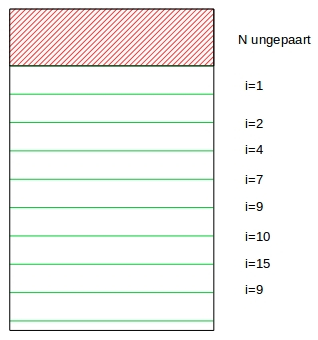
\includegraphics[width=0.5\textwidth]{lectures/160425/pix/4.jpg} & nicht alle i da nicht immer Paarungen möglich\\
\end{tabular}
\\\\
\\\\
 - stochastisch: Zufallszahl zwischen [0,1] = r\\
 - Grenze = $Z(1,n) \cdot r$\\
 - aufsummieren bis $\sum \limits_{0 \leq i <n} x_i > Z \cdot r$ mit i= Bindungspaarungspartner\\
\\\\
Backtracking von:\\
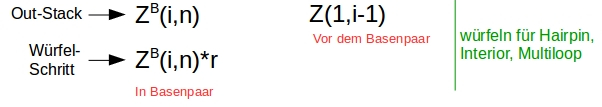
\includegraphics[width=1\textwidth]{lectures/160425/pix/5.jpg}
\\\\
\begin{equation}
Z^B(i,j)= \underbrace{\overbrace{\mathcal{H}(i,j)}^{Energie}}_{Hairpin} + \underbrace{\sum\limits_{i < k < l < j} \overbrace{\mathcal{I}(i,j, k, l)}^{Energie} \cdot \overbrace{Z^B(k,l)}^{auf Stack}}_{Interior} +  \underbrace{\sum\limits_{i < u < j} \overbrace{Z^M(i+1,u)}^{auf Stack} \cdot \overbrace{Z^{M1}(u+1,j-1)}^{auf Stack}}_{Multiloop}
\end{equation}
\\\\
 - schnell für einzelne Strukturen (linear)\\
 - bietet die Möglichkeit Strukturen auf einzelne Eigenschaften zu testen\\
 - findet suboptimale Strukturen (wie Zuker und Wuchty)